\documentclass[twoside,12pt,openany]{report}

%% ===================================================
%% Geometry: Page margins matching TIET specifications
%% ===================================================
\usepackage[
  inner=1.5in,
  outer=1in,
  top=1.8in,
  bottom=0.85in
]{geometry}

\setlength{\emergencystretch}{1.5em}
\widowpenalty=10000
\clubpenalty=10000

%% ===================================================
%% Required Packages
%% ===================================================
\usepackage{fancyhdr}
\usepackage{titlesec}
\usepackage[hidelinks]{hyperref}
\usepackage{graphicx}
\graphicspath{{figures/}}
\usepackage{amsmath}
\usepackage{amssymb}
\usepackage{xcolor}
\usepackage{booktabs}
\usepackage{tabularx}
\usepackage{array}
\usepackage{pdfpages}
\usepackage{pdflscape}

\newcolumntype{L}[1]{>{\raggedright\arraybackslash}p{#1}}

%% ===================================================
%% TIET Report Customizations (Self-Contained in TeX)
%% ===================================================
\makeatletter
\newcommand{\@tpHeader}{UCS503P - Software Engineering Project}
\newcommand{\@tpTitle}{ClassPulse}
\newcommand{\@tpSubTitle}{A Real-Time Classroom Engagement Platform}
\newcommand{\@tpAuthors}{%
  \begin{tabular}{@{}r@{\hspace{1.2em}}l@{}}
    \texttt{1024030691} & Priyam Goel \\
    \texttt{1024030768} & Rahil Yadav \\
    \texttt{1024030660} & Aksh Kaushik \\
    \texttt{1024030664} & Chinmay
  \end{tabular}%
}
\newcommand{\@tpSubText}{Group: 3C75, BE Third Year, COE}
\newcommand{\@tpAdvisor}{Dr. Nisha Thakur}
\newcommand{\@tpFooter}{%
  \large End-Semester Evaluation \\[0.2cm]
  \bfseries Computer Science and Engineering Department \\[0.15cm]
  Thapar Institute of Engineering and Technology, Patiala%
}

% Configuration commands
\newcommand{\TitlePageHeader}[1]{\renewcommand{\@tpHeader}{#1}}
\newcommand{\ProjectTitle}[1]{\renewcommand{\@tpTitle}{#1}}
\newcommand{\ProjectSubTitle}[1]{\renewcommand{\@tpSubTitle}{#1}}
\renewcommand{\author}[1]{\renewcommand{\@tpAuthors}{#1}}
\newcommand{\TitlePageSubText}[1]{\renewcommand{\@tpSubText}{#1}}
\newcommand{\AdvisorName}[1]{\renewcommand{\@tpAdvisor}{#1}}
\newcommand{\TitlePageFooterText}[1]{\renewcommand{\@tpFooter}{#1}}

% Fancyhdr headers and footers (page numbers removed from all pages)
\pagestyle{fancy}
\fancyhf{}
\setlength{\headheight}{15pt}
\fancyhead[LE]{\@tpHeader}
\fancyhead[RO]{\@tpTitle}
\renewcommand{\headrulewidth}{0.5pt}
\renewcommand{\footrulewidth}{0pt}

% Ensure plain style (used on chapter start pages and TOC) has no page numbers
\fancypagestyle{plain}{%
  \fancyhf{}%
  \renewcommand{\headrulewidth}{0pt}%
  \renewcommand{\footrulewidth}{0pt}%
}

% Titlesec custom chapter heading format
\titleformat{\chapter}[display]
  {\raggedleft\bfseries\large}
  {Chapter \thechapter}
  {0.3em}
  {\huge}
  [\vspace{0.1em}\hrule]
\titlespacing*{\chapter}{0pt}{-50pt}{40pt}
\assignpagestyle{\chapter}{empty}

% Maketitle definition
\renewcommand{\maketitle}{%
  \begin{titlepage}
    \thispagestyle{empty}
    \centering
    \vspace*{0.5cm}

    {\large \textbf{\@tpHeader}}

    \vspace{2cm}
    {\LARGE \textbf{\@tpTitle}}

    \vspace{0.2cm}
    {\@tpSubTitle}

    \vspace{3.5cm}
    {\large \textbf{Submitted by:}}

    \vspace{0.2cm}
    {\large \@tpAuthors}

    \vspace{0.5cm}
    {\normalsize \@tpSubText}

    \vfill

    {\large \textbf{Submitted to:}}

    \vspace{0.2cm}
    {\normalsize \@tpAdvisor}

    \vspace{0.8cm}
    
\includegraphics[width=2.9cm]{tiet_logo.png}

    \vspace{0.6cm}
    {\normalsize \@tpFooter}
  \end{titlepage}

  \newpage
  \thispagestyle{empty}%
}
\makeatother

%% ==================================================
%% PROJECT METADATA & CONFIGURATION
%% ==================================================

\TitlePageHeader{%
  UCS503P - Software Engineering Project%
}

\ProjectTitle{%
  ClassPulse%
}

\ProjectSubTitle{%
  A Real-Time Classroom Engagement Platform%
}

\author{%
  \begin{tabular}{@{}r@{\hspace{1.2em}}l@{}}
    \texttt{1024030691} & Priyam Goel \\
    \texttt{1024030768} & Rahil Yadav \\
    \texttt{1024030660} & Aksh Kaushik \\
    \texttt{1024030664} & Chinmay
  \end{tabular}%
}

\TitlePageSubText{%
  Group: 3C75, BE Third Year, COE%
}

\AdvisorName{%
  Dr. Nisha Thakur%
}

\TitlePageFooterText{{%
    \large End-Semester Evaluation \\[0.2cm]
    \bfseries Computer Science and Engineering Department%
  } \\[0.15cm]
  Thapar Institute of Engineering and Technology, Patiala%
}

%% ==================================================

\begin{document}

% Generate title page
\maketitle

% Table of contents (auto-generated from chapters)
\addtocontents{toc}{\protect\footnotesize}
\tableofcontents

% ==================================================
% CHAPTER 1: INTRODUCTION
% ==================================================

\chapter{Introduction}

\section{Background and Context}

Most undergraduate engineering courses still rely on large lectures. A section can have sixty to over a hundred students, and the teacher has to teach, watch for confusion, manage attendance, and answer questions at the same time. Two problems keep coming up. The first is \emph{attendance integrity}: how do we know who is actually in the room without using up class time or accepting proxy entries? The second is \emph{engagement visibility}: how does the teacher know whether students are following the lecture, where they are stuck, and which doubts are still open? ClassPulse aims to close this loop with live signals instead of guesses or delayed messages.

Traditional attendance methods force a choice between speed and trust. A roll call in a large class can take 10--15 per cent of the lecture. Paper sheets interrupt the class, are easy to manipulate, and have to be entered into a system later. Static QR codes and shared links are faster, but they do not expire and are not tied to a device. A student who is present can photograph the code or forward the link, and an absent friend can mark attendance from outside the hall. The records are late and unreliable, and they tell the teacher nothing until the class is over.

The engagement problem is just as real. In a one-way lecture, students who lose track rarely stop the class to ask a question, and a quiet room is not necessarily a room that understands. Classroom-response tools, online quiz platforms, and LMS forums each solve a small part of the problem, but they are separate products with separate logins and separate class lists. A teacher who wants a quick poll, a short quiz, and a place for doubts has to set up several tools, and students have to install several apps for one course. Doubt groups often move to \mbox{WhatsApp}, where they are hard to search, get repeated, and make students hesitant to ask basic questions.

ClassPulse treats attendance and engagement as two parts of the same class session. It has a web dashboard for teachers, a Flutter app for Android students, and an installable web app for iOS and other devices. The base is an anti-proxy attendance flow: the teacher projects a short-lived sequence of signed QR codes, and the student app has to scan it within a strict time window. On top of that, the final system adds PulseMeter live feedback, teacher-made quizzes with server-timed scoring and leaderboards, a pseudonymous doubt forum with scoped search, and analytics that bring attendance, participation, quiz scores, and doubt activity together.

The mid-semester review covered the attendance base and the identity, classroom, and roster services that the other modules need. This report covers the completed end-semester system: how the attendance flow was hardened, how PulseMeter, quizzes, the forum, search, and analytics were built and connected, and how the whole platform was tested.

\subsection{Problem Statement}

Attendance capture and classroom engagement in physical and hybrid courses therefore suffer from several connected deficiencies:

\begin{itemize}
  \item \textbf{Proxy-prone attendance:} Static QR codes, shared links, and paper sheets do not prove that a student is in the room at that moment. An absent student can use a forwarded screenshot or link, so the record may not match who was actually present.
  \item \textbf{Loss of instructional time:} Roll calls, passing sheets around, and fixing roster mistakes eat into lecture time. The problem gets worse in larger classes, which are exactly the classes where reliable records matter most.
  \item \textbf{Delayed pacing feedback:} Teachers get no live signal about whether the class is following. They usually find out only after an assessment, when the lecture has already moved on.
  \item \textbf{Passive participation:} Students are often reluctant to admit confusion or ask a question in front of the whole class. Without an easy channel, the teacher never sees that uncertainty.
  \item \textbf{Fragmented, unsearchable doubts:} Questions asked in class or in \mbox{WhatsApp} groups disappear after the session. There is no easy way to check whether a doubt has already been answered, so the same questions come up again.
  \item \textbf{No unified engagement view:} Attendance, polls, quizzes, and discussions sit in different tools. Class lists are duplicated, participation cannot be compared with attendance, and the teacher cannot see who is present and how the class is responding in one place.
  \item \textbf{No self-service attendance visibility:} Students cannot easily check their own attendance or see how close they are to the minimum requirement. They usually find out about a shortfall only when it is reported formally.
\end{itemize}

ClassPulse brings these needs into one role-based platform. Teachers create classrooms, start attendance sessions, launch live activities, author quizzes and PulseMeters, and review analytics. Students join with a code or link, scan the QR sequence, answer live activities and timed quiz questions, and take part in pseudonymous discussions. A Node.js backend handles login, permissions, attendance rules, live activity state, quiz timing, and forum visibility. PostgreSQL stores the permanent records, and Redis keeps only the short-lived attendance state.

The platform only needs an Android phone, a laptop with a browser, and the classroom projector, so no special hardware is required. It uses well-known methods---HMAC-signed time tokens, PostgreSQL full-text search, and standard web and mobile frameworks---instead of new cryptography or search research. This keeps the focus on getting the workflow and real-time behaviour right.

\section{Project Objectives}

The end-semester objectives take the attendance prototype and turn it into a complete classroom platform. Each objective can be checked in the deployed system through a functional or end-to-end test.

\begin{enumerate}
  \item \textbf{Secure, role-based multi-platform architecture:} Build a teacher web dashboard, a Flutter Android app, and an installable student web app. Use JWT login, bcrypt password hashing, and role checks so each user can only do what their role allows.

  \item \textbf{Classroom and enrollment management:} Let teachers create sections from a fixed course list, generate unique join codes and shareable links, and manage the class list. Let students join, view, and leave a classroom during the semester.

  \item \textbf{Anti-proxy dynamic QR attendance:} Generate rotating HMAC-SHA256-signed QR frames for each session. Accept only a complete, correctly ordered scan within 10 seconds, validate it through Redis, prevent duplicate attendance, and record Attendance Capture Latency (ACL) for every accepted scan. Aim for a median ACL of 10 seconds or less during evaluation.

  \item \textbf{PulseMeter live feedback:} Let teachers create reusable word-cloud, MCQ, and rating-scale activities and launch one at a time in a class. Show live totals and present-versus-responded participation, and allow a student to be muted from word clouds for 7 to 180 days after an inappropriate response.

  \item \textbf{Live MCQ quizzing:} Support teacher-made MCQ quizzes with server-controlled timing and time-weighted \mbox{WIDE} or \mbox{NARROW} scoring. Show answer distributions after each question and keep a live leaderboard that produces a final result.

  \item \textbf{Pseudonymous doubt forum with audience-scoped search:} Provide threaded doubts at classroom, course, and app level. Include topic tags, replies, accepted solutions, helpful marks, teacher endorsement, and a per-course pseudonym. Let users search past doubts, but only within the audience they are allowed to see.

  \item \textbf{Cross-feature analytics and reporting:} Give teachers attendance trends, per-student detail, ACL averages, quiz and PulseMeter participation, and an engagement overview. Give students per-subject attendance against the 75\% requirement. Support manual attendance correction, CSV and Excel export, and low-attendance warnings.

  \item \textbf{Deployment, quality, and end-to-end validation:} Run automated CI for the backend, web app, and Flutter app; deploy on managed cloud services with PostgreSQL and Redis; distribute the Android build; test full teacher--student workflows; and evaluate the system through the planned classroom pilot or a simulated pilot, reporting ACL, participation, and doubt-resolution results.
\end{enumerate}

% ==================================================
% CHAPTER 2: METHODOLOGY AND DESIGN
% ==================================================

\chapter{Methodology and Design}

\section{System Architecture}

ClassPulse uses a three-tier client-server design. The presentation tier has the teacher dashboard and the student apps. The application tier has the REST API and the real-time service. The data tier has PostgreSQL for permanent data and Redis for short-lived state. Each tier can be developed, tested, and deployed on its own, and the connections between them are clearly defined.

The teacher dashboard is built with Next.js~\cite{nextjs}. It handles classroom creation, class lists, attendance sessions, QR projection, PulseMeter and quiz authoring, live results, forum moderation, and analytics. Students use either the Flutter Android app or the installable student web app. The Android app supports camera scanning and a mobile attendance view. The web app gives students the same main features on devices where the Android build is not available.

The backend is a Node.js and Express service. It provides REST endpoints for login, classrooms, enrollment, attendance, PulseMeter, quizzes, doubts, search, and analytics. Socket.io~\cite{socketio} sends session events such as attendance check-ins, live activity launches, response totals, question starts, and leaderboard changes. The backend also enforces permissions, input checks, rate limits, and the rules that the client should not be trusted to enforce.

PostgreSQL is the main store for users, courses, classrooms, enrollments, attendance, live activities, quizzes, forum content, and search data. Redis only holds short-lived data, such as the current QR batch for an active session. This keeps permanent records safe in PostgreSQL while the fast, temporary attendance checks stay in Redis.

\subsection{High-Level Design}

A normal interaction starts with login. The client sends credentials over HTTPS. The backend checks the password against its bcrypt hash and returns a signed JSON Web Token (JWT)~\cite{rfc7519}. Every protected request carries this token. Middleware checks the signature and expiry, then attaches the user's identity and role to the request. Role checks then limit what the user can do.

Classrooms are tied to a fixed course list. A teacher picks a course code and creates a section with a unique six-character join code. Students join with the code or a shareable link. A uniqueness rule stops the same student from joining the same section twice, so the class list can be used for both attendance and live activities.

Attendance is the most time-sensitive flow. When a teacher starts a session, the backend creates the session and a batch of three QR tokens. Each token carries the session ID, batch ID, sequence number, timestamp, a random token ID, and an HMAC-SHA256 signature~\cite{rfc2104}. The dashboard shows the three codes in order and fetches a new batch before the old one expires. A student scans all three in order, and the app sends the sequence with the device scan-start time. The backend checks the structure, order, batch, age, signatures, Redis entry, session, enrollment, and any earlier record before it saves attendance. The teacher's class list updates over Socket.io without a refresh.

Live activities use the same real-time channel. A teacher launches a saved PulseMeter or quiz, and the system creates one active activity for that classroom. A database rule allows only one active activity per class at a time. Student responses are saved in PostgreSQL, and the class sees totals rather than individual answers. For quizzes, the server stores the start and end time of each question, so scoring does not depend on the student's clock.

The doubt forum uses normal request-response calls. A post is visible to an app-wide, course-wide, or classroom audience and is tagged with a course topic. Replies, helpful marks, accepted solutions, endorsements, and reports are stored separately, with uniqueness rules that stop duplicate votes. Search uses a generated \texttt{tsvector} column and a GIN index. The same audience rule used for viewing a post is also used in search, so search cannot reveal a post the user is not allowed to open.

\begin{landscape}
\begin{figure}[p]
  \centering
  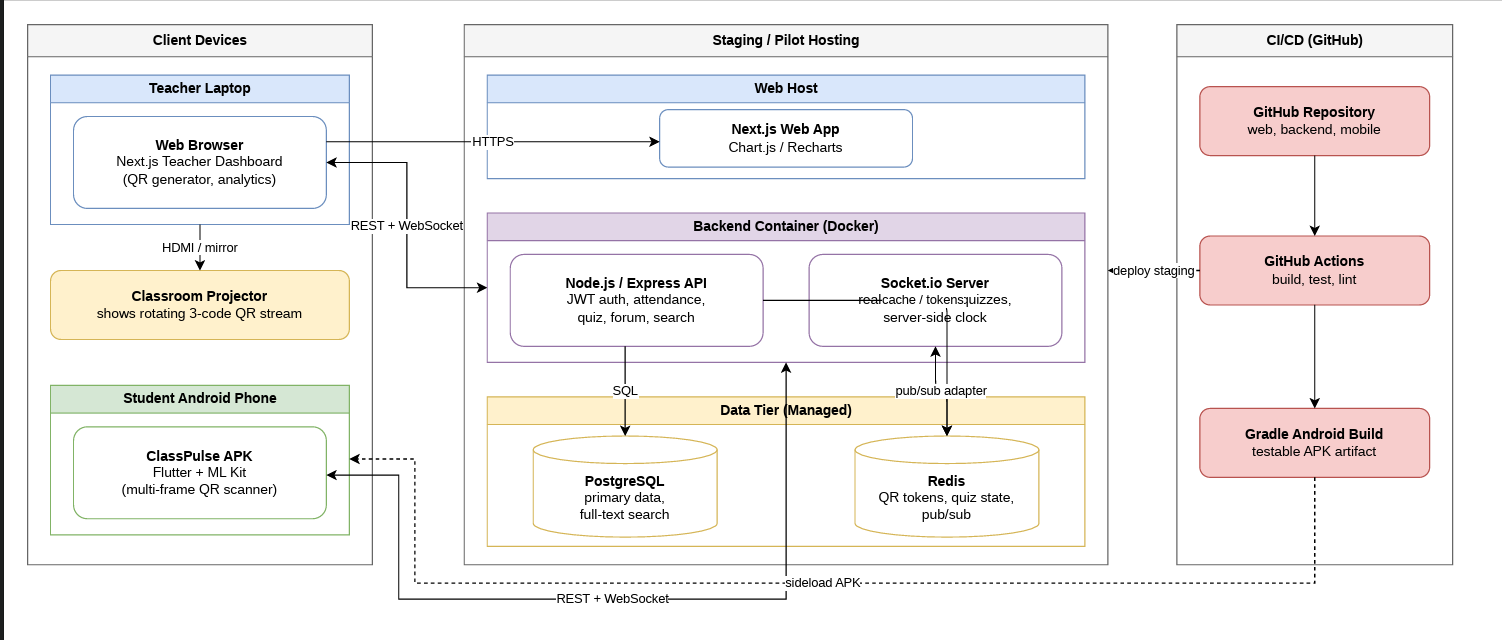
\includegraphics[width=\linewidth]{deployment_diagram.png}
  \caption{Deployment Diagram}
  \label{fig:deployment}
\end{figure}
\end{landscape}

\subsection{Technical Stack}

The implementation uses mature, widely available components rather than custom infrastructure. Table~\ref{tab:stack} summarises the stack.

\begin{table}[htbp]
  \centering
  \small
  \caption{Technical Stack}
  \label{tab:stack}
  \begin{tabularx}{\textwidth}{@{}L{2.6cm}L{4.4cm}X@{}}
    \toprule
    \textbf{Layer} & \textbf{Technology} & \textbf{Responsibility} \\
    \midrule
    Instructor web & Next.js 14, React, TypeScript, MUI v5 & Dashboard, authoring, QR projection, live results, forum moderation, analytics \\
    Student web & Next.js PWA, self-hosted WASM QR decoder & Installable iOS/Android client with attendance, activities, quizzes, and forum \\
    Student mobile & Flutter, Dart, Material 3 & Native Android client with camera scanning and attendance dashboard \\
    Backend & Node.js 20, Express.js & REST API, authentication, validation, business rules, exports, notifications \\
    Real time & Socket.io with Redis adapter & Session rooms, attendance events, live activity updates, leaderboards \\
    Database & PostgreSQL (Neon) & Durable relational storage and native full-text search \\
    Cache & Redis (Upstash) & Short-lived QR batches, token validation state, pub/sub \\
    Charts & Recharts (web), \texttt{fl\_chart} (mobile) & Attendance, ACL, participation, and quiz visualisations \\
    Delivery & GitHub Actions, Render, Vercel, Firebase & CI, backend hosting, web hosting, Android APK distribution \\
    \bottomrule
  \end{tabularx}
\end{table}

PostgreSQL fits because most of the data is relational: a classroom belongs to a course and a teacher, students join through enrollments, attendance belongs to a session, and replies belong to posts. Foreign keys, check constraints, and unique constraints enforce many rules directly in the database. PostgreSQL full-text search means we do not need a separate search service, and the audience check stays in the same query as the search.

Redis is used only for data that can disappear. A QR batch lives for 15 seconds, and tokens older than 10 seconds are rejected anyway. Keeping this in Redis avoids a database write for every rotation and makes validation a quick cache lookup. Socket.io provides the live updates, and its Redis adapter leaves room to run more than one backend instance.

The web and mobile apps share Material Design 3 values. The dashboard uses MUI with those values, and the Flutter app uses Material 3 directly. This keeps colours, type, shapes, and elevation consistent. Recharts and \texttt{fl\_chart} provide the same kind of charts on web and mobile.

\subsection{Deployment and Runtime Environment}

The deployed system uses managed services so the team can focus on the application. Next.js runs on Vercel, and the Express/Socket.io service runs in a container on Render. PostgreSQL is on Neon, Redis is on Upstash, and Android test builds go through Firebase App Distribution. GitHub Actions runs the backend tests, the web test and build, and the Flutter analysis, tests, and APK build.

The application tier is stateless. User identity is carried in signed tokens, not server memory. Live activity state that must survive a restart is stored in PostgreSQL. Only QR batches live in Redis. This makes the backend easy to replace and allows the real-time layer to scale through the Redis adapter.

\section{UML and System Models}

The design is shown with UML and structured-analysis diagrams. The use case and class models describe the static structure, while the sequence, activity, and data flow diagrams show how the main workflows move data and events through the system.

\subsection{Use Case Model}

There are two human actors. The \textbf{Instructor} creates and manages sections, starts attendance, authors and launches activities, moderates the forum, and views analytics. The \textbf{Student} joins sections, scans attendance, responds to PulseMeters, takes quizzes, and takes part in pseudonymous discussions. Both use the same login, but role checks decide which actions they can perform.

\begin{figure}[htbp]
  \centering
  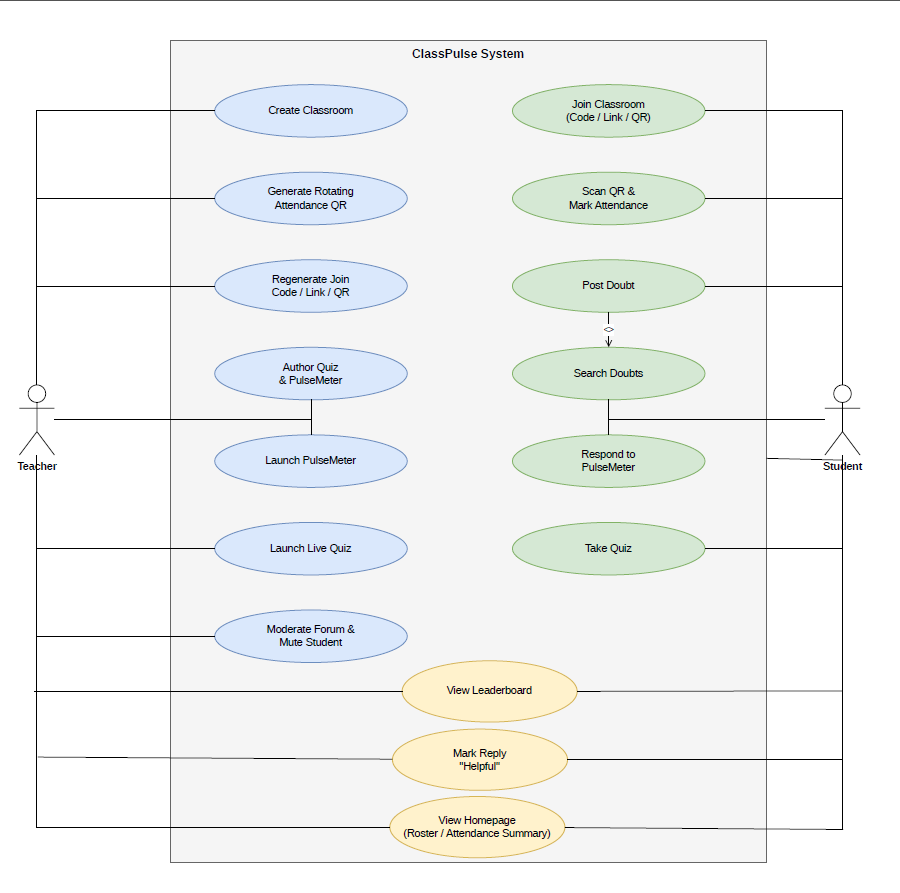
\includegraphics[width=0.78\textwidth]{use_case_diagram.png}
  \caption{Use Case Diagram}
  \label{fig:use_case}
\end{figure}

\begin{table}[htbp]
  \centering
  \footnotesize
  \renewcommand{\arraystretch}{0.95}
  \caption{Principal Use Cases}
  \label{tab:use_cases}
  \begin{tabularx}{\textwidth}{@{}L{1.3cm}L{5.6cm}L{2.4cm}X@{}}
    \toprule
    \textbf{ID} & \textbf{Use Case} & \textbf{Primary Actor} & \textbf{Outcome} \\
    \midrule
    UC-01 & Register and authenticate & Instructor, Student & A valid JWT and role-scoped session \\
    UC-02 & Create and configure a classroom & Instructor & Section with a unique join code \\
    UC-03 & Join a classroom & Student & Enrollment in the section roster \\
    UC-04 & Start and end an attendance session & Instructor & Active session and rotating QR batch \\
    UC-05 & Scan attendance QR sequence & Student & One validated PRESENT record and ACL value \\
    UC-06 & Author a PulseMeter or quiz & Instructor & Reusable activity definition \\
    UC-07 & Launch and respond to a PulseMeter & Instructor, Student & Combined live feedback and participation \\
    UC-08 & Attempt a live quiz & Student & Timed answer and time-weighted score \\
    UC-09 & View live quiz results and leaderboard & Instructor, Student & Answer distribution, score, and rank \\
    UC-10 & Post, reply, search, and mark doubts helpful & Instructor, Student & Scoped discussion and retrievable answer \\
    UC-11 & View analytics and export attendance & Instructor, Student & Trends, drill-downs, and report files \\
    UC-12 & Moderate content & Instructor & Muted word-cloud author or flagged forum content \\
    \bottomrule
  \end{tabularx}
\end{table}

\begin{figure}[htbp]
  \centering
  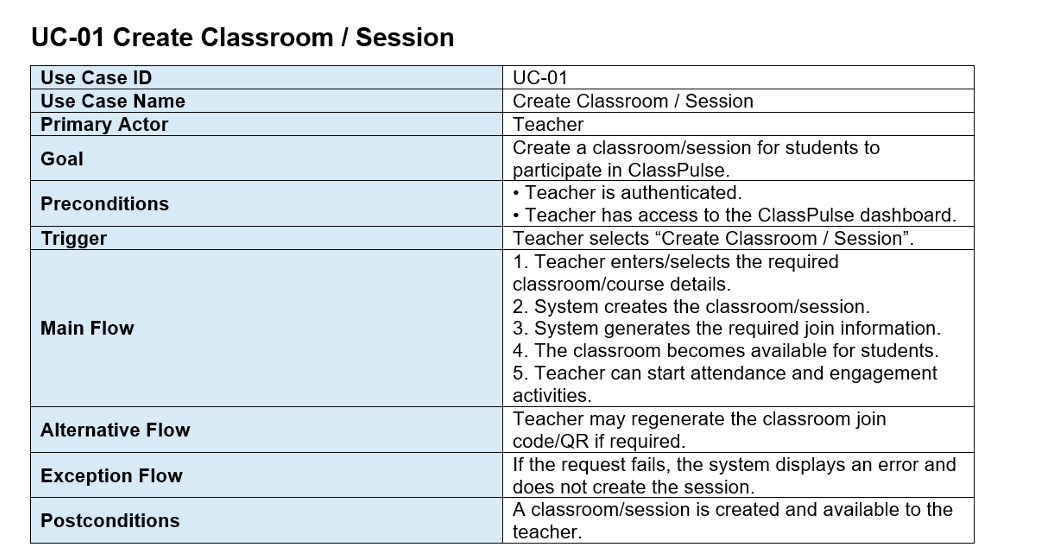
\includegraphics[width=0.92\textwidth]{use_case_uc01.png}\\[0.4em]
  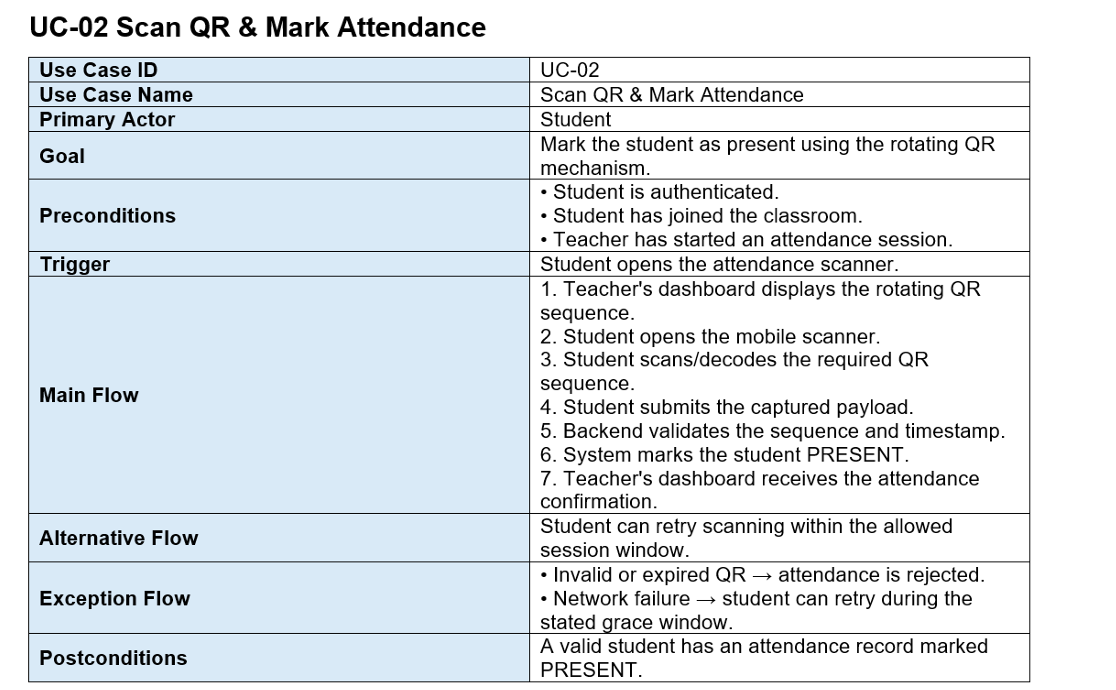
\includegraphics[width=0.92\textwidth]{use_case_uc02_clean.png}
  \caption{Use Case Templates: (a) Create Classroom/Session and (b) Scan QR and Mark Attendance}
  \label{fig:use_case_templates}
\end{figure}

\subsection{Class Diagram}

The class model follows the database schema. A \texttt{Course} has many \texttt{Classrooms}. A \texttt{Classroom} belongs to one \texttt{Teacher} and has many \texttt{Enrollments}. A \texttt{Student} has many \texttt{Enrollments}. A \texttt{Classroom} has many attendance \texttt{Sessions}, and each session has many \texttt{AttendanceRecords}. A \texttt{LiveActivity} points to either a \texttt{PulseMeter} or a \texttt{Quiz}, and responses belong to the activity and the student. Forum posts, replies, helpful marks, and reports form a separate but connected model.

\begin{figure}[p]
  \centering
  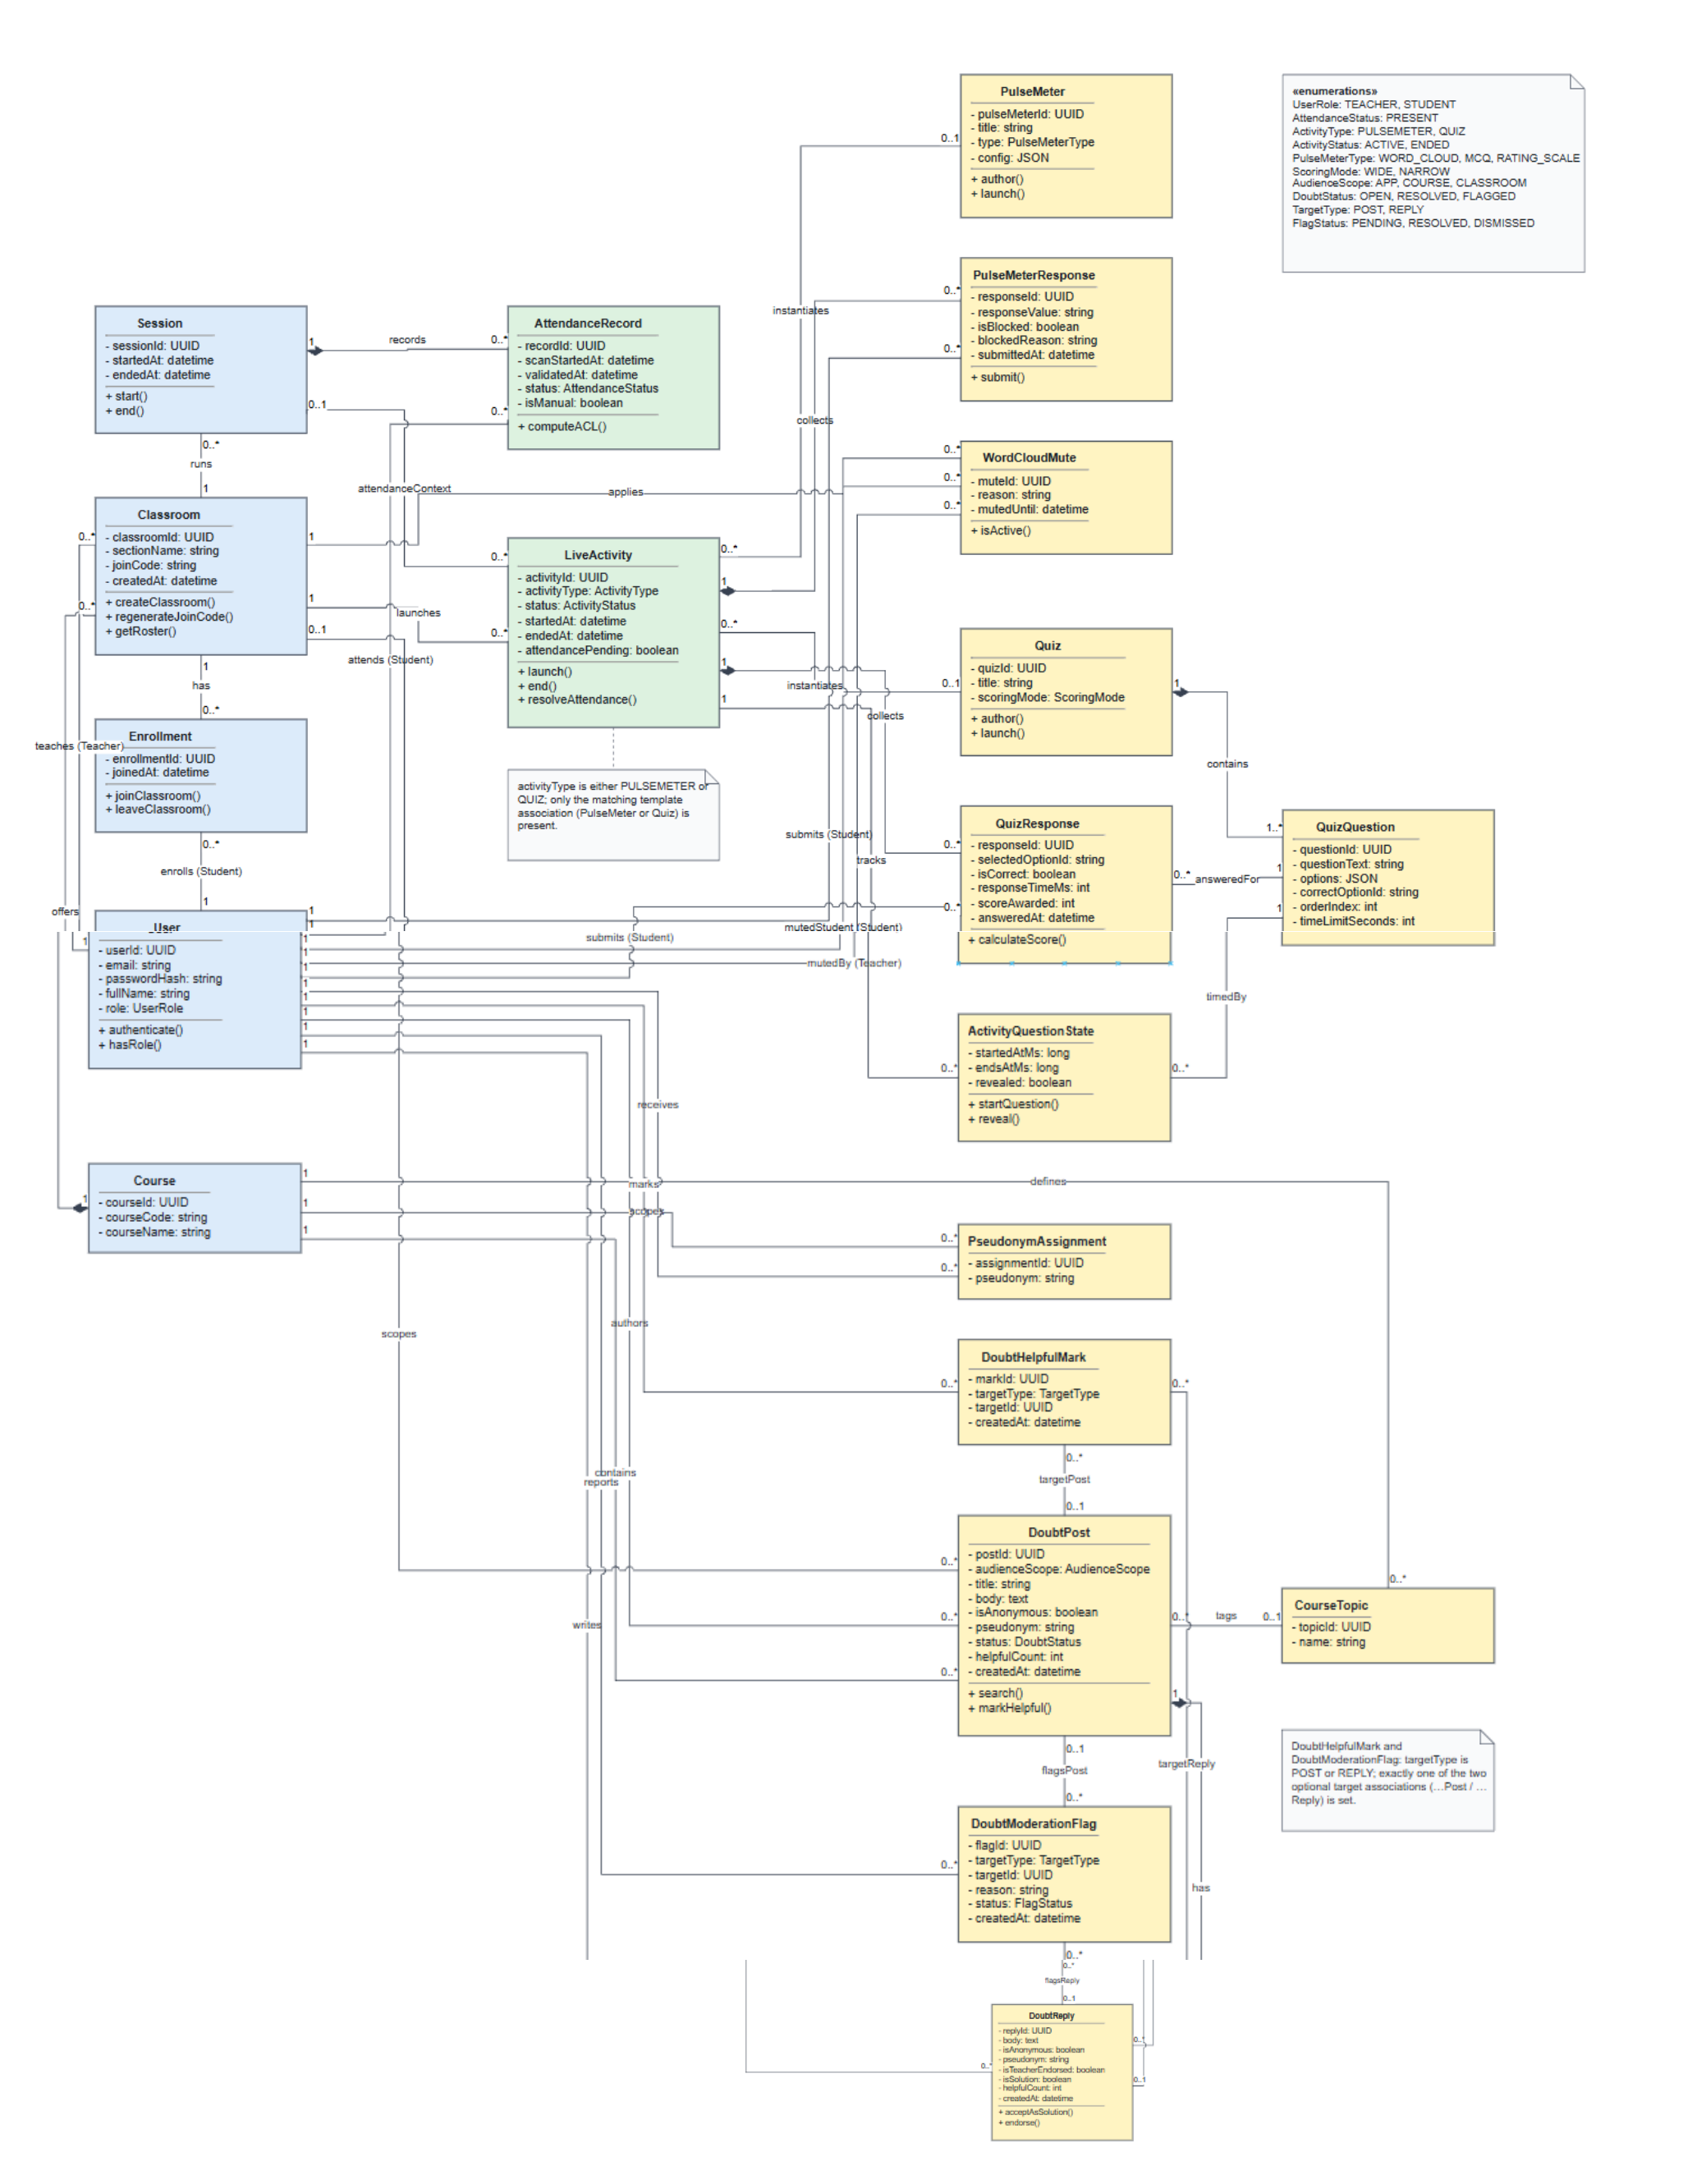
\includegraphics[height=0.88\textheight,keepaspectratio]{class_diagram.png}
  \caption{Class Diagram}
  \label{fig:class_diagram}
\end{figure}

\subsection{Sequence Diagram}

Figure~\ref{fig:seq_attendance} shows the attendance flow. The teacher starts a session, the backend creates the session and a three-token batch, and the dashboard shows the frames. The student app scans the three frames, sends them with a scan-start time, and gets a result. The backend then saves the attendance record and sends the live class-list update.

\begin{figure}[htbp]
  \centering
  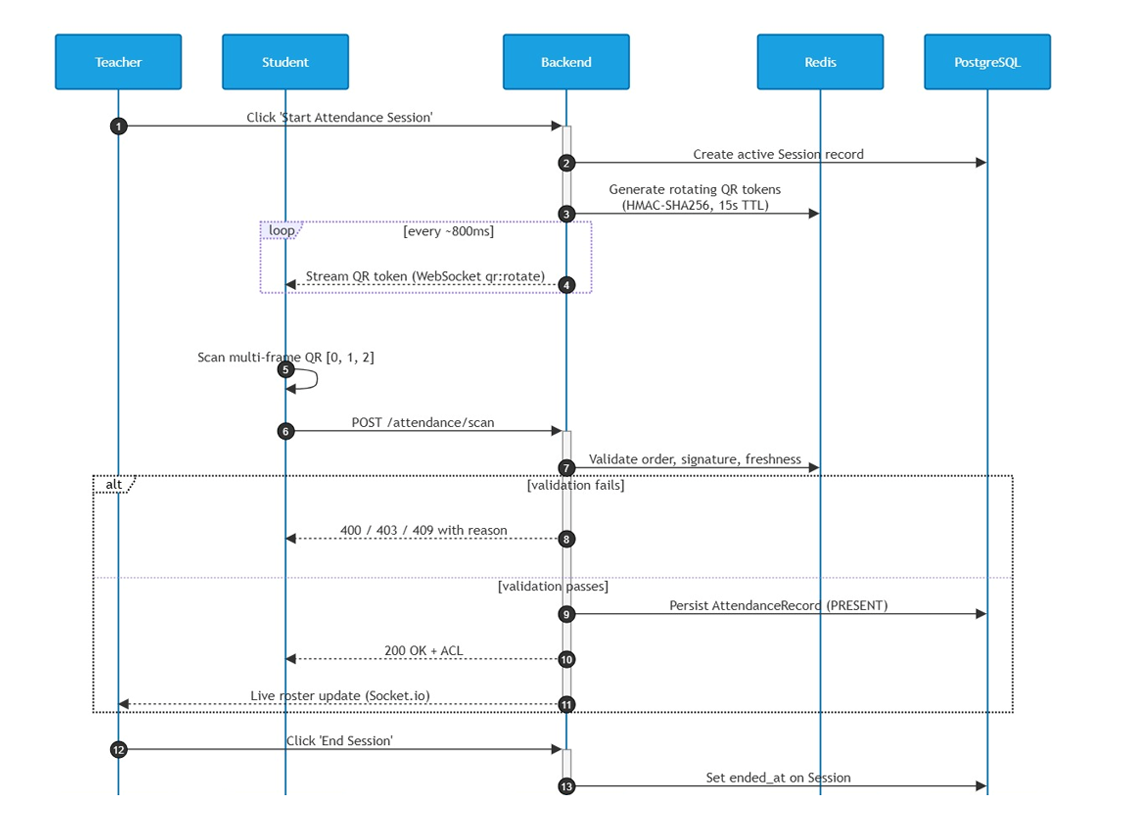
\includegraphics[width=0.95\textwidth]{sequence_attendance_clean.png}
  \caption{Sequence Diagram: Attendance Verification}
  \label{fig:seq_attendance}
\end{figure}

\subsection{Activity Models}

Figure~\ref{fig:activity_auth} shows login and role routing. Figure~\ref{fig:activity_classroom} shows classroom creation and student enrollment. Figure~\ref{fig:activity_attendance} shows the checks that decide whether a scan is accepted: the session is active, all three frames are present, the order is correct, the batch matches, the timestamp is fresh, the signature is valid, the Redis entry exists, the student is enrolled, and there is no earlier record. If any check fails, the flow ends without saving attendance.

\begin{figure}[htbp]
  \centering
  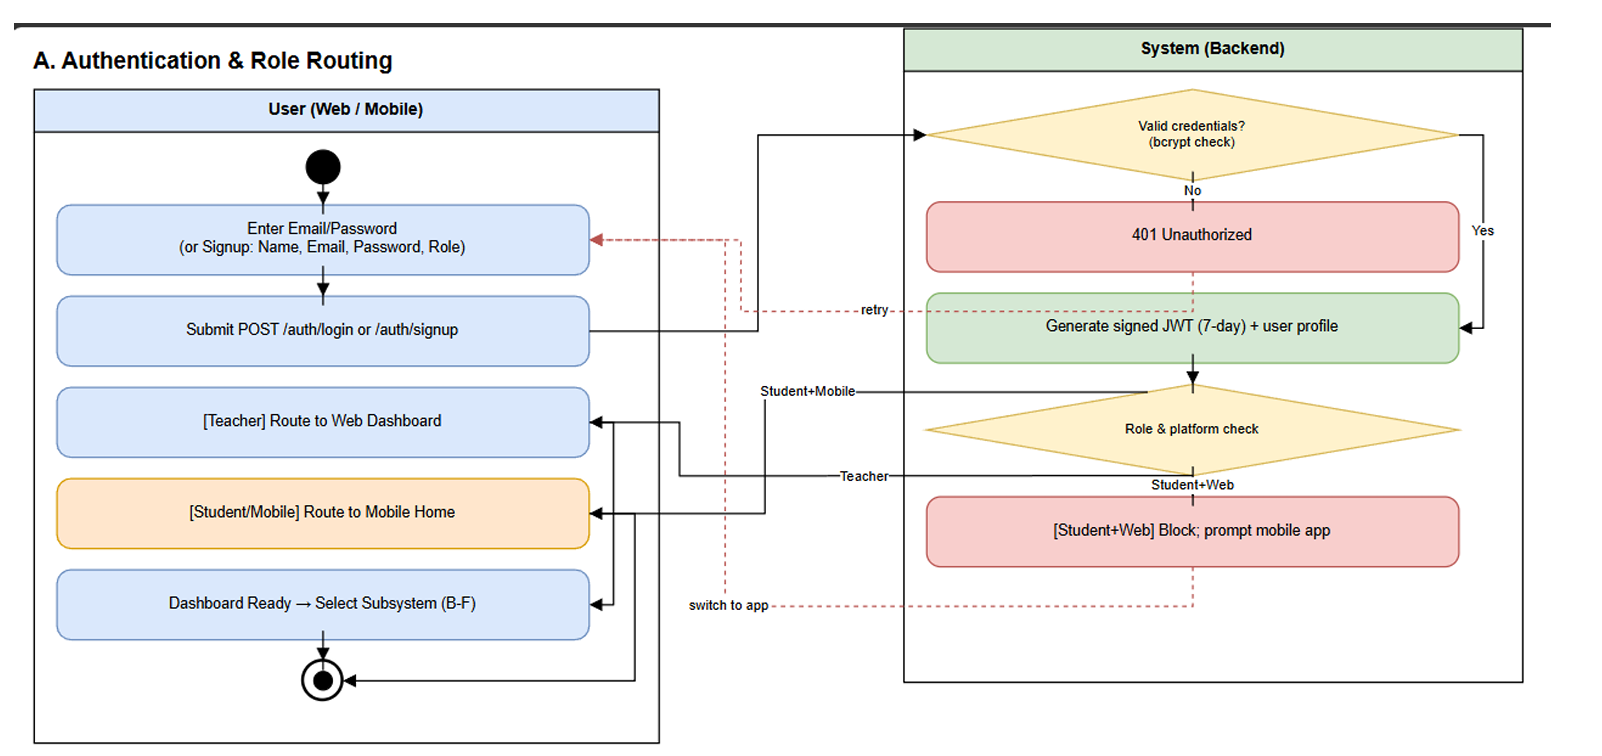
\includegraphics[width=\textwidth]{activity_auth.png}
  \caption{Activity Diagram: Authentication and Role Routing}
  \label{fig:activity_auth}
\end{figure}

\begin{figure}[htbp]
  \centering
  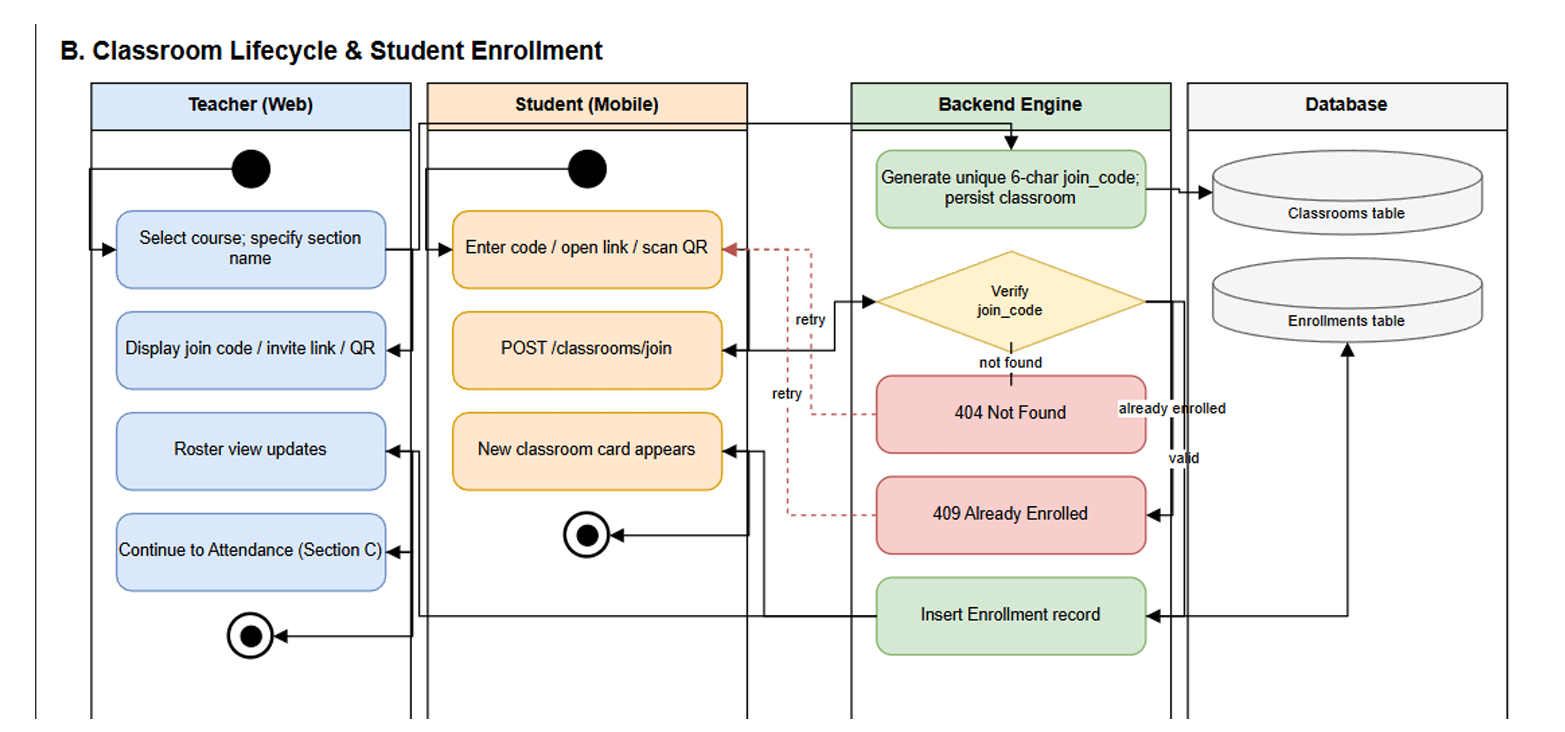
\includegraphics[width=\textwidth]{activity_classroom.png}
  \caption{Activity Diagram: Classroom Lifecycle and Student Enrollment}
  \label{fig:activity_classroom}
\end{figure}

\begin{figure}[htbp]
  \centering
  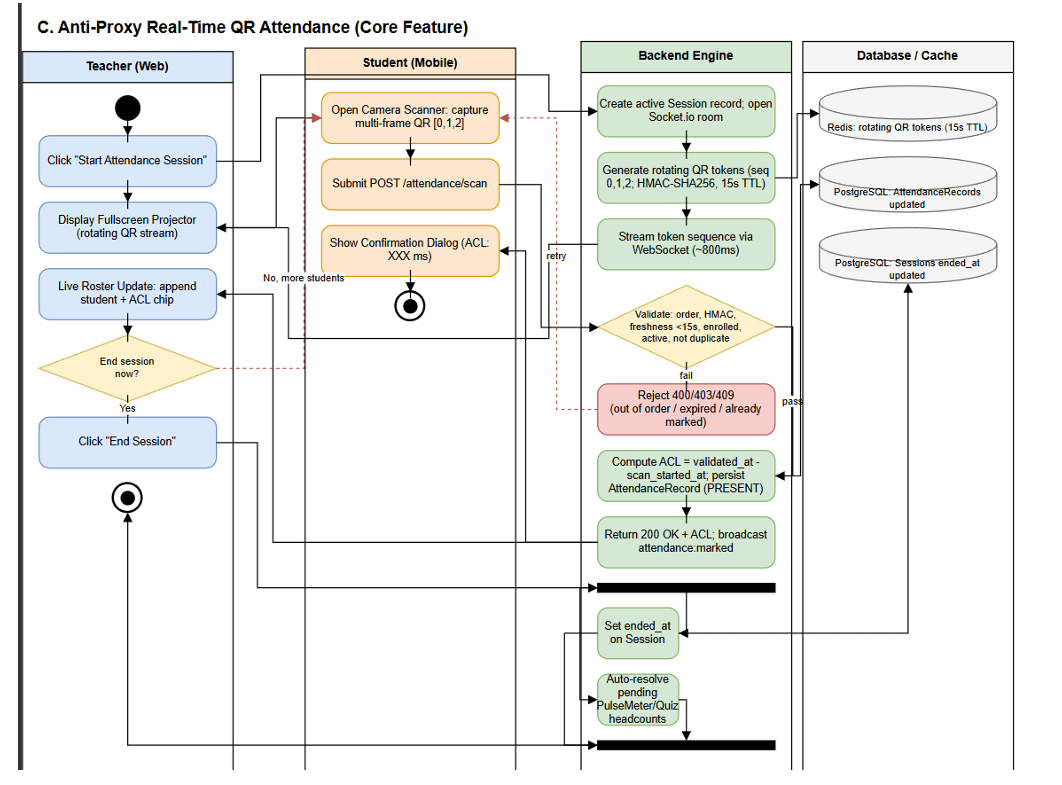
\includegraphics[width=0.92\textwidth]{activity_attendance.png}
  \caption{Activity Diagram: Anti-Proxy QR Attendance}
  \label{fig:activity_attendance}
\end{figure}

A live activity has a short lifecycle. It starts as \texttt{ACTIVE} when launched, stays as the only active activity in its classroom, and becomes \texttt{ENDED} when the teacher closes it. A pending PulseMeter may later use an attendance session to work out its present count.

\subsection{Data Flow Diagrams}

The level-0 diagram treats ClassPulse as one process with three external entities: the teacher, the student, and the cloud services that store data and carry live updates. The level-1 diagram splits the system into login and classroom management, attendance, live activities, forum and search, and analytics.

\begin{figure}[htbp]
  \centering
  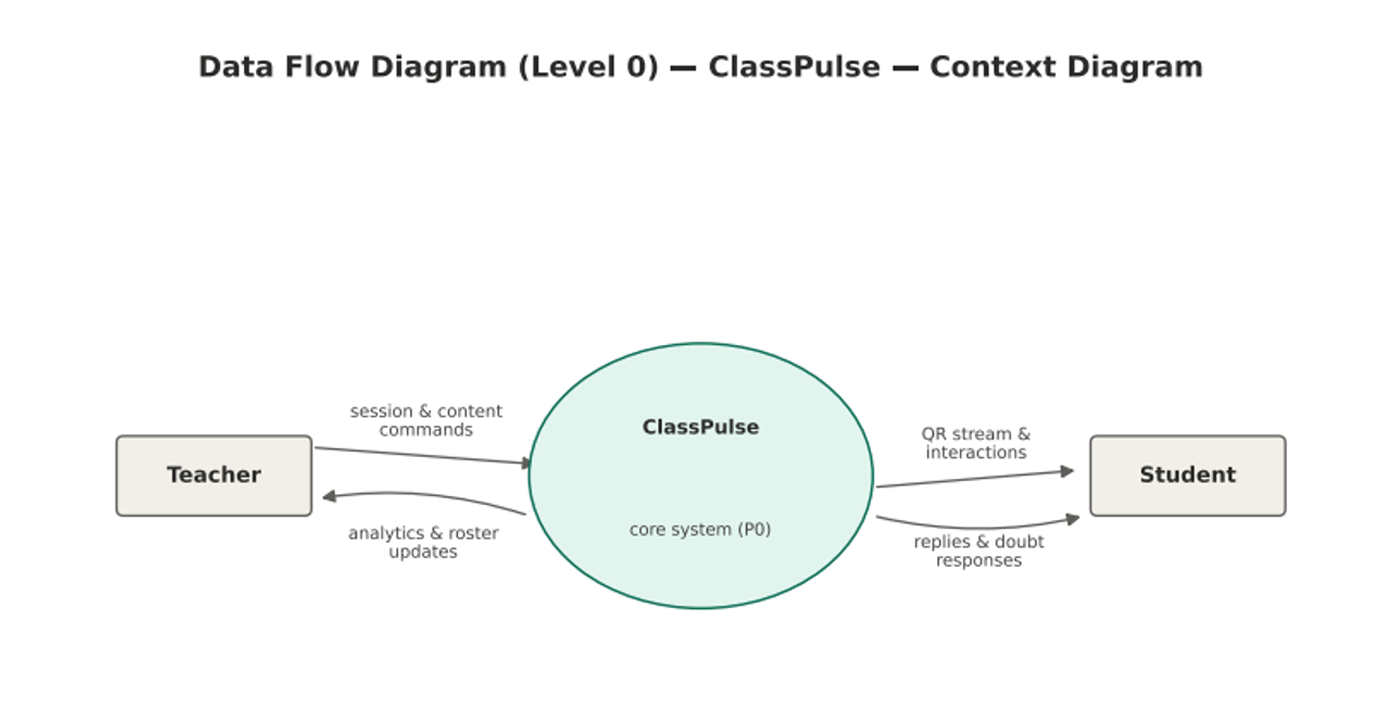
\includegraphics[width=0.95\textwidth]{dfd_level0.png}
  \caption{Level 0 Data Flow Diagram}
  \label{fig:dfd0}
\end{figure}

\begin{figure}[htbp]
  \centering
  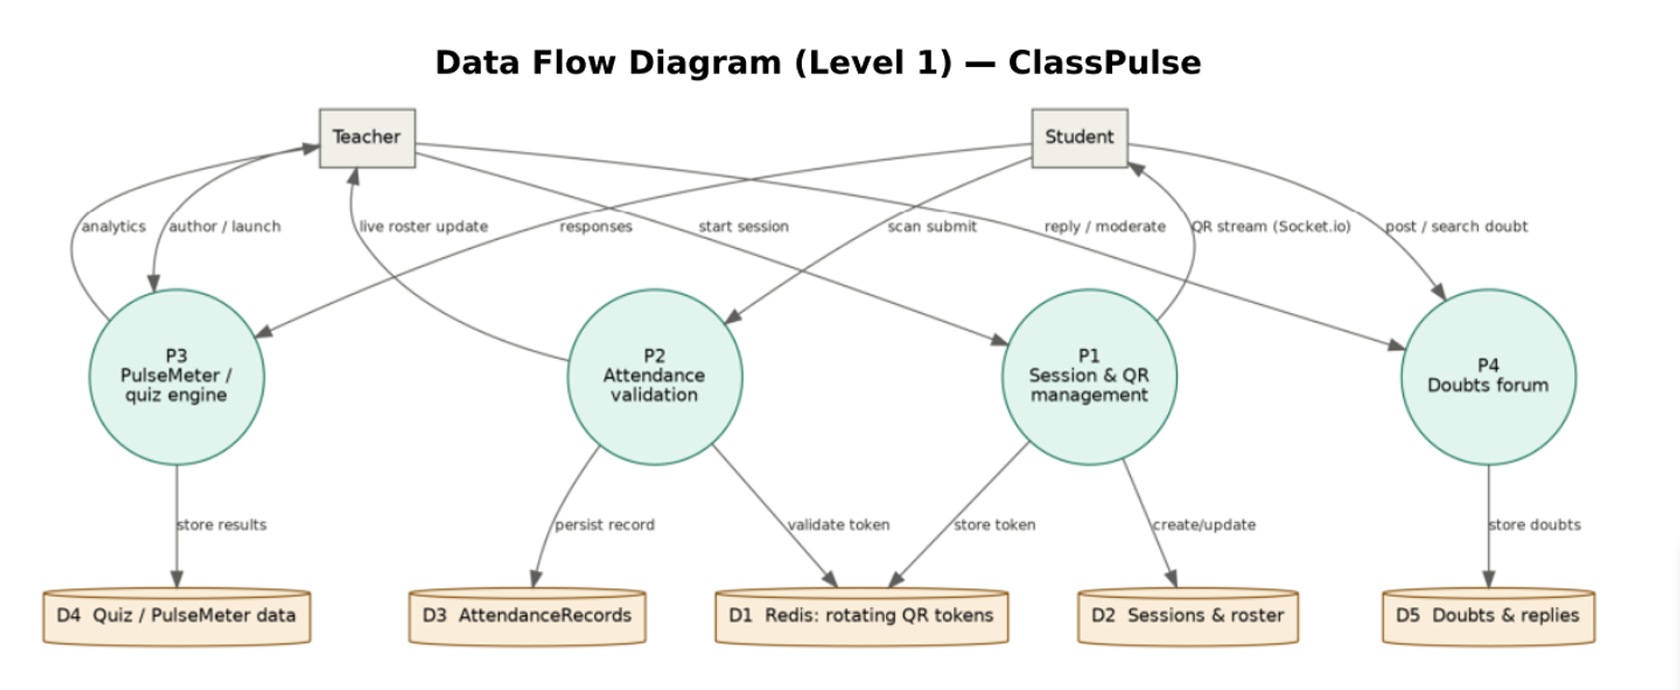
\includegraphics[width=\textwidth]{dfd_level1_clean2.png}
  \caption{Level 1 Data Flow Diagram}
  \label{fig:dfd1}
\end{figure}

\section{Implementation Details}

\subsection{Identity, Roles, and Enrollment}

Passwords are hashed with bcrypt~\cite{provos1999} before they are stored and are never returned by the API. Login returns a signed JWT with the user ID and role. Middleware checks the token on protected routes, and role checks block teacher-only actions. Student actions are also checked against enrollment, so a student cannot read or change another section's data.

Teachers create sections from a fixed course list to avoid variants like ``UCS101'' and ``UCS 101''. Each section gets a six-character join code and a uniqueness check. Join links carry the same code. A unique rule on classroom and student prevents duplicate joins, even if two requests arrive at the same time.

\subsection{Anti-Proxy Attendance Pipeline}

A session's QR batch has three tokens with sequence numbers 0, 1, and 2. The signed payload ties together the session, batch, sequence number, timestamp, and a random token ID. The HMAC-SHA256 signature stops a client from making up a sequence, and the random ID stops an old payload from being replayed. The compact JSON keeps the QR code easy to project and scan.

The batch is cached in Redis under a session key with a 15-second expiry. The server accepts a batch only while it is within the 10-second freshness window; the extra 5 seconds give a scan already in progress time to finish. A batch can be reused for a short interval so that polling does not change the codes faster than students can scan them.

Validation follows a fixed order. The backend checks the shape of the request, then the sequence, batch, timestamp, signatures, Redis entry, session, enrollment, and earlier attendance. It saves an \texttt{attendance\_records} row only after every check passes. The unique rule on session and student gives one last guard against two submissions arriving together. Capture latency is calculated as

\begin{equation}
  \mathrm{ACL} = \texttt{validated\_at} - \texttt{scan\_started\_at},
\end{equation}

\noindent Here the first timestamp comes from the backend, and the second is captured on the student's device when scanning starts. Manual teacher corrections are stored with \texttt{is\_manual = TRUE} so that ACL statistics can leave them out.

\subsection{PulseMeter Live Feedback}

A PulseMeter is created once and reused. Its type is \texttt{WORD\_CLOUD}, \texttt{MCQ}, or \texttt{RATING\_SCALE}, and its settings are stored as JSONB. Launching it creates a live activity and sends it to the classroom room. A partial unique index stops two activities from running at the same time in one class.

Each student can respond once per activity. Word-cloud answers are cleaned and counted by frequency; MCQ answers are counted by option; rating answers are counted by value. The live view shows totals, not raw answers. A profanity filter can block a word-cloud entry when it is submitted, and a teacher can mute a student from future word clouds for a set period. The mute belongs to the classroom and has an expiry time.

PulseMeter analytics separate \emph{present} from \emph{responded}. If an attendance session has already ended for the lecture, the activity is linked to it and the present count becomes the denominator. If attendance is not final yet, the activity is marked pending. When the attendance session ends, pending activities for that classroom are resolved and their analytics are recalculated. This avoids showing a participation rate against a class size that is not settled.

\subsection{Live Quiz Engine}

A quiz has a title, a scoring mode, and an ordered list of MCQs. Each question stores its options, correct option, order, and time limit. When a question starts, the backend saves the official start and end time in \texttt{activity\_question\_states}. The student payload leaves out the correct option, and only the latest question accepts answers.

For a correct answer, let $T$ be the question time limit and $t$ the server-measured response time. The remaining-time fraction is

\begin{equation}
  f = \max\left(0, \min\left(1, \frac{T - t}{T}\right)\right).
\end{equation}

\noindent WIDE mode gives $300 + 700f$ points, and NARROW mode gives $700 + 300f$ points. A wrong answer gets zero. Scores are saved per response, so the leaderboard is built from stored rows rather than a counter in memory. On reveal, the backend sends the correct option and answer distribution, and the cumulative leaderboard is sorted by total score.

\subsection{Doubt Forum and Audience-Scoped Search}

A doubt post is visible to an \texttt{APP}, \texttt{COURSE}, or \texttt{CLASSROOM} audience. Classroom posts carry a classroom ID; course and app posts do not. Each post also has a predefined course topic, which keeps labels consistent across students. Replies are separate rows, and a reply can be marked as the accepted solution or endorsed by the teacher.

Pseudonyms are scoped to a course and stay the same for that student. The backend creates the pseudonym from an HMAC of the user and course IDs and saves it, so a student keeps one pseudonymous name across posts in a course without revealing their real name. Helpful marks sit in their own table with a uniqueness rule on user and target, which stops repeated voting. Reports are also stored separately, so a teacher can review flagged content without deleting the discussion.

Search uses a generated \texttt{tsvector} column~\cite{postgresfts}. The title has weight \texttt{A} and the body \texttt{B}, and a GIN index keeps retrieval fast. Queries use \texttt{plainto\_tsquery}, rank results with \texttt{ts\_rank}, and build a headline with \texttt{ts\_headline}. The audience check runs in the same query as the text match, so search cannot expose a post the user is not allowed to see.

\subsection{Analytics, Reporting, and Notifications}

The analytics layer uses the same tables as the live features. Teachers see section attendance, session turnout, per-student detail, average ACL, quiz performance, PulseMeter participation, and doubt activity. Students see per-subject attendance, a comparison with the 75\% requirement, and session history. Web charts use Recharts, and mobile charts use \texttt{fl\_chart} with the same Material 3 values.

Attendance can be exported as a CSV or Excel matrix. Teachers can correct attendance when needed, and the record is marked so that scan-based ACL numbers stay clean. Low-attendance warnings use the same percentage calculations and can be emailed through the configured mail provider. These features keep the platform useful after the live session, instead of treating analytics as a separate reporting product.

\subsection{Student Clients and Installable Web Application}

The Flutter app uses the phone camera and a barcode-scanning library~\cite{flutter,mlkit} to read QR frames. It keeps a three-frame buffer, sends the scan only when all frames are present and in order, and shows the returned ACL straight away. It also handles classroom joining, attendance history, PulseMeter responses, quizzes, and the doubt forum.

The student web app gives the same main workflow on iOS and other devices where the Android build is not available. It uses a self-hosted WebAssembly QR decoder, so scanning does not depend on a native camera plugin, and it stores the session token locally for authenticated requests. Both student apps use the same light-mode Material 3 design as the teacher dashboard.

% ==================================================
% CHAPTER 3: RESULTS AND EVALUATION
% ==================================================

\chapter{Results and Evaluation}

\section{Testing Methodology}

Testing was done at four levels. \emph{Unit tests} cover small pieces such as token generation, login helpers, scoring, exports, profanity filtering, email sending, and client utilities. \emph{Integration tests} call route handlers with controlled database and Redis dependencies, including permission failures and duplicate requests. \emph{End-to-end tests} run complete teacher--student workflows on the deployed apps. \emph{Static and build checks} confirm that the web app type-checks and builds and that the Flutter app passes analysis and widget tests.

The automated tests are part of CI. The backend job installs dependencies, checks syntax, and runs the Node test runner. The web job runs Vitest, type-checks, and builds the production app. The mobile job runs Flutter analysis, unit and widget tests, and builds an Android APK. The pipeline runs on changes, so the same checks are repeated before delivery.

Functional testing used the four end-to-end cases in Appendix A. Each case has a normal path and at least one failure or boundary check. They cover login and section creation, joining a class, the QR attendance flow, and live quiz scoring. They were designed on 11 November 2026 and run against the deployed system on 15 November 2026.

\section{Test Environment and Execution}

Table~\ref{tab:testenv} summarises the environment used for functional execution.

\begin{table}[htbp]
  \centering
  \small
  \caption{Functional Test Environment}
  \label{tab:testenv}
  \begin{tabularx}{\textwidth}{@{}L{3.5cm}X@{}}
    \toprule
    \textbf{Component} & \textbf{Configuration} \\
    \midrule
    Instructor web client & Production deployment on Vercel \\
    Backend API & Production deployment on Render \\
    Database & Neon PostgreSQL with the production schema \\
    Cache and real-time state & Upstash Redis \\
    Student mobile client & Flutter Android build distributed to testers \\
    Student web client & Installable Next.js PWA \\
    Browser & Chromium-based browser for the instructor dashboard \\
    Execution date & 15 November 2026 \\
    \bottomrule
  \end{tabularx}
\end{table}

The automated tests were also run locally while preparing this report. Table~\ref{tab:automated} shows the results. These are counts of tests that ran, not a coverage estimate.

\begin{table}[htbp]
  \centering
  \small
  \caption{Automated Test Results}
  \label{tab:automated}
  \begin{tabularx}{\textwidth}{@{}L{3.2cm}L{5.0cm}X@{}}
    \toprule
    \textbf{Suite} & \textbf{Command} & \textbf{Observed Result} \\
    \midrule
    Backend & \texttt{npm test} & 213 tests passed, 0 failed \\
    Web & \texttt{npm test} (Vitest) & 29 tests passed across 6 files, 0 failed \\
    Mobile & \texttt{flutter test} & 13 tests passed, 0 failed \\
    Static analysis & \texttt{flutter analyze --no-fatal-infos} & No error-level findings; 5 informational style notices \\
    \bottomrule
  \end{tabularx}
\end{table}

\section{Functional Test Results}

All four cases passed. Table~\ref{tab:functional} gives the summary, and Appendix A has the full steps, expected responses, and post-conditions. All 28 steps passed on the deployed system.

\begin{table}[htbp]
  \centering
  \small
  \caption{Functional Test Summary}
  \label{tab:functional}
  \begin{tabularx}{\textwidth}{@{}L{1.0cm}L{5.2cm}L{3.4cm}L{2.4cm}X@{}}
    \toprule
    \textbf{ID} & \textbf{Test Case} & \textbf{Subsystem} & \textbf{Type} & \textbf{Result} \\
    \midrule
    1.1 & Teacher creates a classroom section & Authentication and section management & Happy path & PASS \\
    1.2 & Student joins a classroom with a join code & Classroom enrollment & Happy path and failure & PASS \\
    1.3 & Anti-proxy QR attendance scan & QR attendance & Complex, happy path and failure & PASS \\
    1.4 & Live quiz answer submission and scoring & Live quiz & Happy path & PASS \\
    \bottomrule
  \end{tabularx}
\end{table}

Test Case 1.1 checked that only someone with the teacher invite code can register, that passwords are stored as bcrypt hashes, and that a new section gets a unique six-character join code. It also checked the failure case: a wrong invite code returns HTTP 403 and creates no account.

Test Case 1.2 checked joining with a code, the student's view of the new section, and the teacher's class list. A duplicate join returned HTTP 409, an invalid code returned HTTP 404, and an empty code was blocked in the app before any request. The database ended with exactly one enrollment row.

Test Case 1.3 ran the full attendance flow. Three frames were scanned in order within the time window. The backend checked the structure, order, batch, age, signature, Redis entry, session, and enrollment, then returned HTTP 200 with an ACL value. The teacher's class list updated over Socket.io without a refresh. A two-frame scan was held in the app and created no record. After the session ended, it appeared in analytics.

Test Case 1.4 covered quiz creation and a live run. The live payload did not include the correct option. A correct answer sent in about five seconds scored between 300 and 1000 in WIDE mode. The reveal showed the correct option and distribution, and the leaderboard used the saved score. The case also confirmed that only one activity can be live in a classroom at a time.

\section{Performance and Non-Functional Evaluation}

Table~\ref{tab:metrics} separates what was actually observed from what still needs a larger pilot. The difference matters: a functional test can show that a valid scan is accepted and an invalid one is rejected, but one session cannot give a median latency or prove a drop in proxy attendance.

\begin{table}[htbp]
  \centering
  \small
  \caption{Evaluation Metrics and Evidence}
  \label{tab:metrics}
  \begin{tabularx}{\textwidth}{@{}L{3.3cm}L{3.0cm}X@{}}
    \toprule
    \textbf{Criterion} & \textbf{Target} & \textbf{Observed Evidence} \\
    \midrule
    Attendance freshness & $\leq 10$ s & Three-frame scan accepted within the freshness window; a two-frame scan was not submitted \\
    Attendance Capture Latency & Median $\leq 10$ s & ACL is logged for every accepted scan and returned to the client; the single-session test produced a valid non-negative value, but a pilot-scale median was not established \\
    Join-code integrity & 6 characters, unique & Verified in Test Case 1.1 \\
    Duplicate enrollment & Rejected & HTTP 409 verified in Test Case 1.2, with exactly one row after the attempt \\
    Invalid join code & Rejected & HTTP 404 verified in Test Case 1.2 \\
    Incomplete QR sequence & Rejected & Two-frame scan produced no attendance record in Test Case 1.3 \\
    WIDE quiz score & 300--1000 & Correct answer returned a score in range in Test Case 1.4 \\
    Live roster update & No page refresh & Socket.io update observed in Test Case 1.3 \\
    Automated regression & All tests pass & 213 backend, 29 web, and 13 mobile tests passed \\
    \bottomrule
  \end{tabularx}
\end{table}

The security checks were reviewed against the controls in the code. Passwords use bcrypt, login uses signed JWTs, role middleware blocks teacher-only actions, student routes check enrollment, database queries are parameterised, join codes and enrollments have uniqueness rules, attendance needs a valid HMAC signature and a fresh timestamp, and login endpoints are rate-limited. These controls cover the main threats in the problem statement, but they are not a substitute for a separate security audit.

Reliability relies on database rules, not only on application code. The unique rule on session and student stops duplicate attendance when two requests arrive together. The rule on activity and student stops duplicate PulseMeter responses. The partial unique index on active activities stops two live activities in one class. The rule on quiz activity, question, and student stops duplicate quiz answers. Foreign keys with cascading deletes keep section removal consistent.

\section{Analysis and Discussion}

The results show that the system meets its functional objectives. Login and role separation work on both clients. Classroom creation and enrollment match between the teacher and student views. Attendance accepts only a complete, fresh, correctly ordered, signed sequence and records latency. PulseMeter and quiz sessions update correctly. The forum respects audience scopes, search returns only visible content, and analytics uses the same records as the live features.

The main limitation is scale. The functional cases used one teacher and one student in a controlled section, so they show correctness, not capacity. Sixty to a hundred students scanning in the same ten-second window would create a burst of requests that was not load-tested. The free-tier deployment also cold-starts after idle periods, which affects the first action of a session but not the normal scan path.

The second limitation is the proposal's evaluation metrics. Median ACL and the survey-based proxy-attendance signal need a real classroom pilot. The system records the timestamps for ACL and rejects invalid sequences, but four functional cases cannot give a measured median or a measured fall in proxy attendance. Those claims should wait for the pilot in Chapter 4.

The third limitation is device and room conditions. Camera decoding depends on projection size, focus, light, and distance from the screen. The app has zoom and a multi-frame buffer, but scan reliability still needs a lecture-hall test across devices. Within these limits, the evidence matches the design goals: attendance is verifiable and resistant to simple proxy attempts, the engagement modules share one class list and one session, and analytics reuses live data instead of a separate reporting pipeline.

% ==================================================
% CHAPTER 4: CONCLUSION
% ==================================================

\chapter{Conclusion}

\section{Summary of Work}

This project set out to close the feedback loop between teachers and students in physical and hybrid classes. The mid-semester prototype built the identity, classroom, roster, and anti-proxy attendance base. The end-semester work added PulseMeter live feedback, time-weighted live quizzes, a pseudonymous doubt forum with scoped search, analytics, reporting, moderation, and an installable student web app.

The attendance module now issues a rotating three-frame HMAC-signed QR sequence, checks it against Redis with a 10-second freshness rule, enforces single use and enrollment, and records ACL for every accepted scan. PulseMeter supports word-cloud, MCQ, and rating-scale activities with live totals, present-versus-responded analytics, and teacher moderation. The quiz engine uses server-controlled timing, WIDE and NARROW scoring, answer-reveal distributions, and a saved leaderboard. The forum supports three audience scopes, course-scoped pseudonyms, replies, accepted solutions, helpful marks, endorsements, and PostgreSQL full-text search. Analytics brings attendance, ACL, participation, quiz performance, and doubt activity together, with CSV and Excel export and low-attendance warnings.

The platform runs as a Next.js web app, a Node.js and Express backend, a Flutter Android app, and an installable student PWA, with PostgreSQL and Redis behind them. The repository includes CI for backend tests, web tests and build, Flutter analysis and tests, and Android APK generation.

\section{Key Findings}

\begin{itemize}
  \item \textbf{Anti-proxy attendance works without special hardware.} A three-frame, short-lived, signed sequence can be checked on ordinary phones and a projector. A single forwarded screenshot is not enough, and the freshness rule limits replay.
  \item \textbf{One classroom context keeps things simple.} The same class, class list, and session are used for attendance, PulseMeter, quizzes, and doubts. This avoids duplicate enrollment data and lets participation be compared with presence.
  \item \textbf{Database rules are safer than good intentions.} Unique constraints and a partial unique index stop duplicate attendance, duplicate responses, and two live activities, even when requests arrive together.
  \item \textbf{The server should own the clock.} Saving question start and end times on the server stops a client from changing its response time and makes the leaderboard reproducible.
  \item \textbf{Search must use the same audience rules as the forum.} Applying the same scope check in search and in normal retrieval stops search from leaking private discussions.
  \item \textbf{Correctness and scale are different claims.} The four end-to-end cases and 255 automated tests support correctness. A classroom pilot is still needed for median ACL, scan reliability, and proxy-attendance impact at real class sizes.
\end{itemize}

\section{Future Work and Recommendations}

\begin{enumerate}
  \item \textbf{Classroom pilot and metric study.} Run the platform in one or two sections of about thirty students for a week. Measure median ACL, rejected-scan rate, PulseMeter participation, and doubt resolution within 24 hours, and run the pre/post proxy-attendance survey from the proposal.
  \item \textbf{Load and soak testing.} Simulate sixty to a hundred students scanning in the same window, and measure API latency, Socket.io fan-out, Redis load, and database connections. Use the results to size the backend and tune the polling interval.
  \item \textbf{Scan reliability across devices.} Test projection size, distance, lighting, camera quality, and zoom on a range of Android and iOS devices. Add a clear retry path for an expired code and a guided scan mode for large halls.
  \item \textbf{Deployment hardening.} Replace free-tier cold starts with an always-on instance during pilot weeks, add monitoring and alerts, and define backup and retention rules for attendance and forum data.
  \item \textbf{Accessibility and localisation.} Check both apps for keyboard access, screen-reader labels, contrast, and text scaling, and move interface strings into translation files.
  \item \textbf{LMS integration.} Add a standards-based export or API link so attendance and quiz results can be reconciled with the institute's learning-management system instead of a separate spreadsheet.
  \item \textbf{AI-assisted authoring (stretch goal).} Let a teacher draft quiz or PulseMeter content in an external assistant and paste structured JSON into the authoring screen, with the teacher still in control of the final content.
  \item \textbf{Native iOS app.} The PWA already covers iOS. A native build would allow deeper camera integration and background behaviour if the pilot shows that browser scanning is not good enough.
\end{enumerate}

\section{Final Remarks}

ClassPulse shows that a small, well-built system can solve a real classroom problem without special hardware or new research. The project used well-known methods---HMAC-signed time tokens, database constraints, server-controlled timing, and native full-text search---inside a workflow that runs across two interfaces. The main lesson was that integrity rules belong in the protocol and the database, not only in the screen. A code that looks right in a screenshot does not prove presence, and a score that looks right on a phone does not prove fair timing. The system is now ready for a classroom pilot. The remaining work is mostly about measurement: how it behaves with real students, real devices, and real lecture halls.

% ==================================================
% BIBLIOGRAPHY
% ==================================================

\clearpage
\addcontentsline{toc}{chapter}{Bibliography}
\begin{thebibliography}{99}

\bibitem{rfc2104}
H. Krawczyk, M. Bellare, and R. Canetti.
\newblock HMAC: Keyed-Hashing for Message Authentication.
\newblock RFC 2104, Internet Engineering Task Force, 1997.
\newblock \url{https://www.rfc-editor.org/rfc/rfc2104}

\bibitem{rfc7519}
M. Jones, J. Bradley, and N. Sakimura.
\newblock JSON Web Token (JWT).
\newblock RFC 7519, Internet Engineering Task Force, 2015.
\newblock \url{https://www.rfc-editor.org/rfc/rfc7519}

\bibitem{provos1999}
N. Provos and D. Mazi\`{e}res.
\newblock A Future-Adaptable Password Scheme.
\newblock In \emph{Proceedings of the USENIX Annual Technical Conference}, 1999.

\bibitem{postgresfts}
PostgreSQL Global Development Group.
\newblock PostgreSQL Documentation: Full Text Search.
\newblock \url{https://www.postgresql.org/docs/current/textsearch.html}, accessed November 2026.

\bibitem{socketio}
Socket.IO.
\newblock Socket.IO Documentation.
\newblock \url{https://socket.io/docs/v4/}, accessed November 2026.

\bibitem{flutter}
Google.
\newblock Flutter Documentation.
\newblock \url{https://docs.flutter.dev/}, accessed November 2026.

\bibitem{mlkit}
Google.
\newblock ML Kit: Barcode Scanning.
\newblock \url{https://developers.google.com/ml-kit/vision/barcode-scanning}, accessed November 2026.

\bibitem{nextjs}
Vercel.
\newblock Next.js Documentation.
\newblock \url{https://nextjs.org/docs}, accessed November 2026.

\end{thebibliography}

% ==================================================
% APPENDIX A: TEST CASE SPECIFICATIONS
% ==================================================

\clearpage
\phantomsection
\addcontentsline{toc}{chapter}{Appendix A: Test Case Specifications}
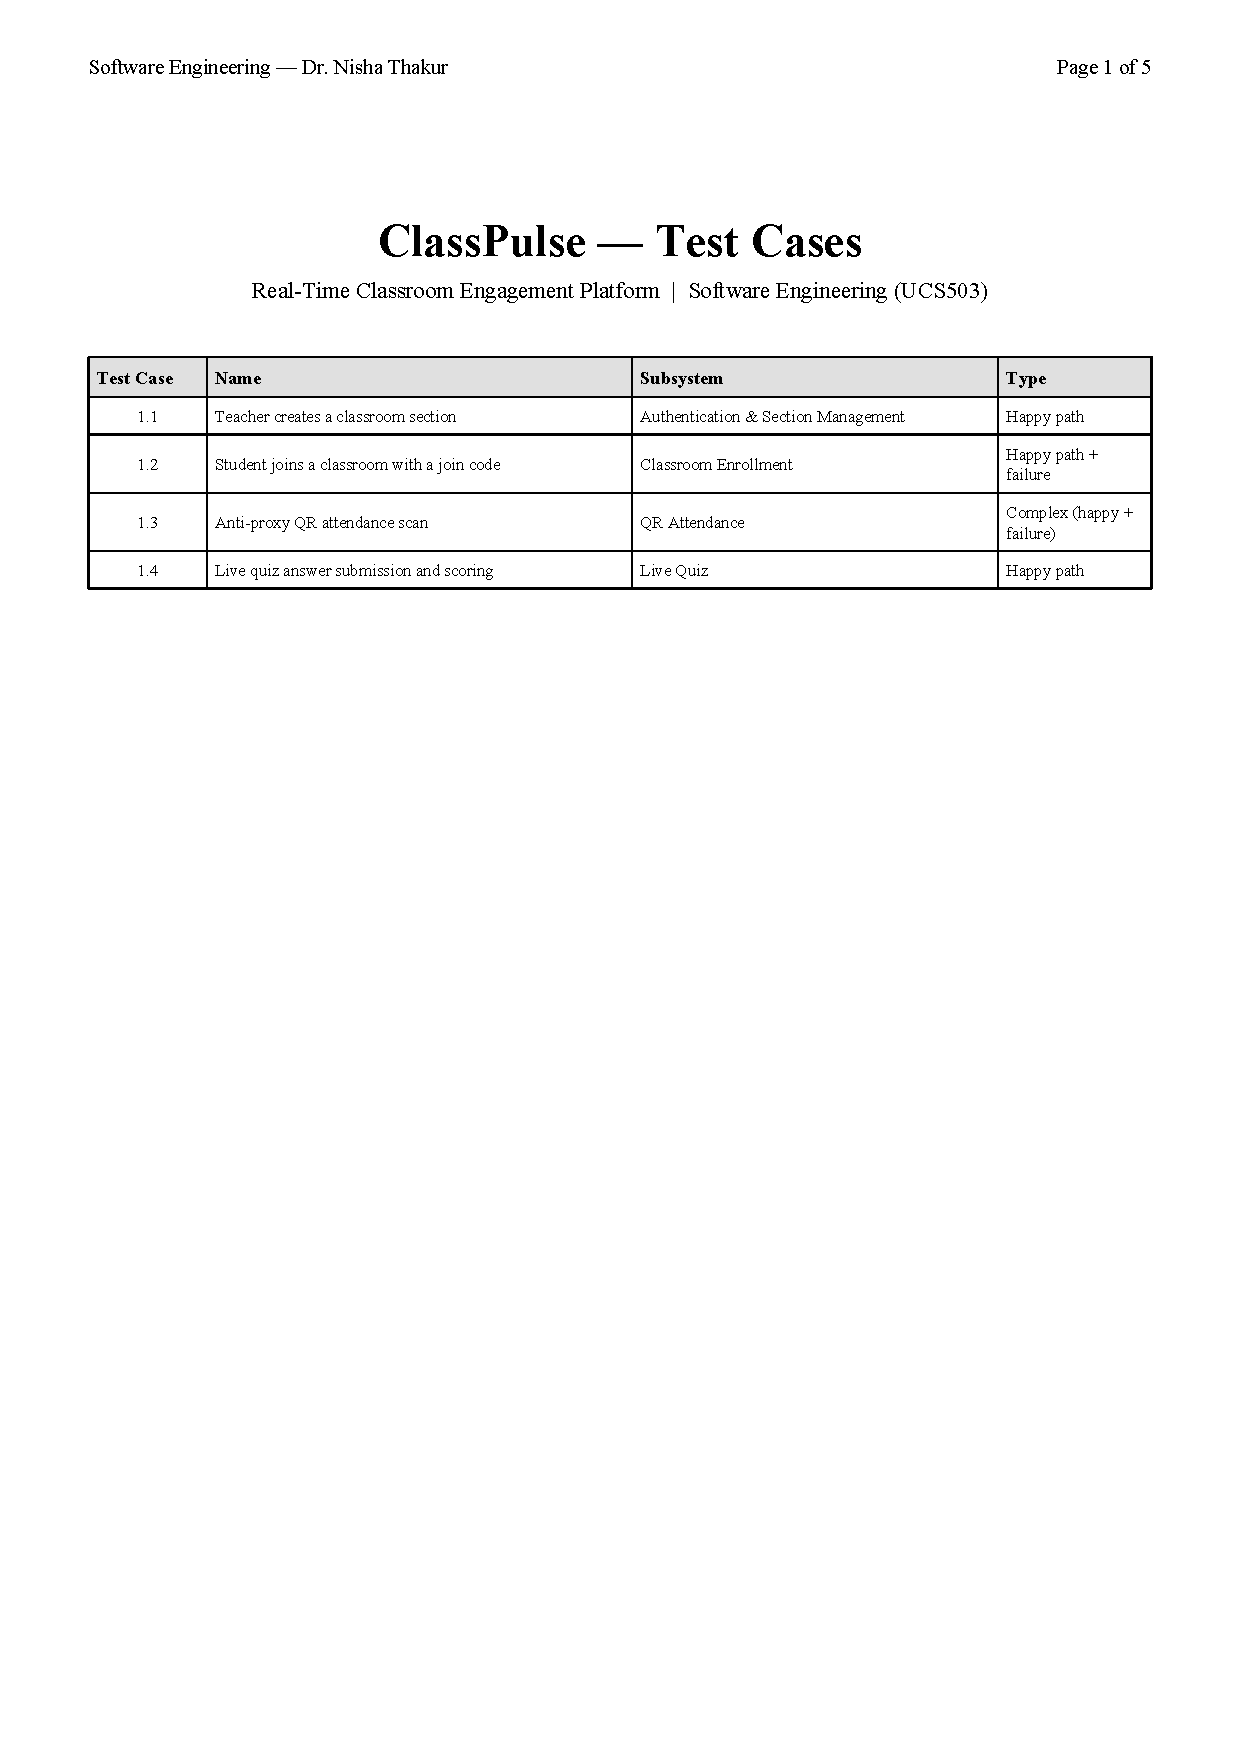
\includepdf[pages=-,pagecommand={\thispagestyle{empty}}]{ClassPulse_Test_Cases_v12.pdf}

\end{document}
